\section{OpenCollab Protocol}
\label{sec:opencollab}

The OpenCollab protocol is implemented by a set of Ethereum smart contracts. By
building on the Ethereum platform, we can rely on security properties of the
underlying Ethereum blockchain. With the details of consensus and security
abstracted away, the OpenCollab protocol focuses on defining secure economic incentives
and rules that encourage open source software sustainability.

\subsection{Protocol Roles}

\begin{itemize}
  \item \textbf{Voters}: participate in governance voting by depositing tokens.
  \item \textbf{Curators}: curate project issues by staking tokens.
  \item \textbf{Contributors}: open pull requests to resolve issues by staking tokens.
  \item \textbf{Maintainers}: review and merge pull requests for issues by
    staking tokens.
\end{itemize}

\subsection{OpenCollab Token}

The OpenCollab token (OCT) powers the OpenCollab protocol. The value offered by
the token is influence over an open source software project. Furthermore, the
token serves the following purposes in the protocol:

\begin{itemize}
  \item Used in deposits for token holders that choose to participate as voters
    in protocol governance.
  \item Used in a staking mechanism for issue curation. Curators stake tokens to
    signal the importance they place on an issue.
  \item Used in a staking mechanism for opening pull requests. Contributors
    stake a certain number of tokens when opening a pull request. If a
    contributor's pull request is closed without being merged in to the project,
    the contributor's staked tokens are destroyed. The possibility of losing
    staked tokens discourages contributors from opening pull requests unless
    they are confident about the quality of their contributions.
  \item Used in a staking mechanism for merging pull requests. Maintainers stake
    a certain number of tokens when they initiate a merge. Before a merge is
    finalized, a token holder can challenge a maintainer's merge to start a
    voting round. If token holders decide to veto a maintainer's merge, the
    maintainer's staked tokens are destroyed. The possibility of losing staked
    tokens discrourages maintainers from merging pull requests that do not
    benefit a project. The challenge and voting process for a merge is described
    in more detail in Section \ref{sec:merge}.
\end{itemize}

An initial allocation of tokens will be distributed so that the various protocol
roles can be fulfilled by token holders. A project creator can initialize an OpenCollab repository and mint a certain amount of
tokens for the initial allocation. The initial allocation might be done using a
token crowdsale or by disbursement at the discretion of the project creator.

OCT is an ERC20 compliant token\cite{erc20} and is divisble by $10^{18}$. When a
repository using the OpenCollab protocol is created, a smart contract is created
governing a OCT that is specific to that particular repository. As a result,
there can be many repository specific versions of OCT.

\subsection{Governance Voting}

Token holders can elect to participate in governance voting by depositing
\textproc{voterDeposit} tokens. At the moment governance voting only takes place
for challenged pull request merges which is described in Section
\ref{sec:merge}, but in the future it can be used for other
protocol decisions. One use case might be to vote on adding maintainers to a
project. Token holders have an incentive to be voters because they stand
to earn rewards if they vote well. Voters on the winning side of a vote increase
their deposits by \textproc{voterRewardPercentage}. At the same time, voters on
the losing side of a vote decrease their deposits by \textproc{voterPenaltyPercentage}.

\subsection{Curating Issues}

Curators stake a number of tokens to an issue to signal the importance that they
place on the issue. Since curators lock up their tokens for a period of time
when they stake tokens to an issue, they have limited curation power. Curators either exchange funds for tokens by purchasing them
on the secondary market or work for tokens by being a
contributor or maintainer. Furthermore, since curators take on the risk of a
fall in token value, they have skin in the game\cite{skininthegame}. If curators
signal importance for bad issues, developers poorly allocate their time and
attention. If developers properly allocate their time and attention on resolving
issues that would increase the quality of a project, the community might lose
interest and less people would desire influence over the project leading to a
fall in token value. Consequently, curators have an incentive to signal
importance for issues that accurately reflect the needs of the community. As
well curated issues are resolved, the value of the token would increase thereby
benefiting curators.

\subsection{Opening Pull Requests}

Contributors open pull requests by staking \textproc{contributorStake} tokens,
where \textproc{contributorStake} is a repository parameter.

If a contributor's pull request is successfully merged by a maintainer, the
contributor receives a portion of the issue's token reward. The portion can be
calculated as \textproc{reward} - (\textproc{reward} $*$ \textproc{maintainerPercentage}).

If a contributor's pull request is closed without being merged into the project,
the contributor's \textproc{contributorStake} staked tokens are destroyed.

\subsection{Merging Pull Requests}
\label{sec:merge}

Maintainers merge pull requests by staking \textproc{maintainerStake} tokens,
where \textproc{maintainerStake} is a repository parameter.

If a maintainer wants to merge a pull request, it calls
\textproc{initMergePullRequest(id)} to signal an intent to merge a particular pull
request and starts a challenge period. During this period, any token holder can
challenge the maintainer by calling \textproc{challenge()} and staking
\textproc{challengerStake} tokens.

If a maintainer is not challenged during the challenge period, he can call
\textproc{mergePullRequest(id)}. The maintainer receives a portion of the
issues's token reward which can be calculated as \textproc{reward} $*$ \textproc{maintainerPercentage}.

If a maintainer is challenged during the challenge period, a voting
period begins. Voting takes place using a two step commit and reveal protocol
first formalized by Brassard, Chaum and Crepeau\cite{proofsofknowledge}. During
the commit step, voters with a minimum \textproc{voterDeposit} deposit in the
smart contract vote to uphold or veto a maintainer's merge by calling
\textproc{commitVote(hash)} with the cryptographic hash of their vote and a secret
phrase. A vote to uphold is a $1$ and a vote to veto is a $2$. The secret phrase
can be any random string only known to the voter. The value of the vote is
secure from an attacker as long as only the voter knows the secret phrase used
when generating the hash. We use the SHA3 \textproc{keccak256} hash function
since it is used internally by Ethereum.

During the reveal step, voters reveal the values of their votes by submitting
the concatenation of their vote and secret phrase used in the commit step by
calling \textproc{revealVote(vote)}. The smart contract verifies that the
submitted vote corresponds with the committed hash and tallies up votes as
voters reveal them. Finally, anyone can call \textproc{voteResult()} which
compares the number of uphold and veto votes. The value that receives the
majority of vote ($\geq 50\%$) wins. Voters on the losing side of the vote are
penalized such that \textproc{voterPenaltyPercentage} is deducted from their
deposits. Voters on the winning side of the vote are rewarded such that
\textproc{voterRewardPercentage} is added to their deposits.

If a maintainer's merge decision is upheld, the maintainer is able to call
\textproc{mergePullRequest(id)} to finalize the merge. The challenger's
\textproc{challengerStake} staked tokens are destroyed and the maintainer can
claim his portion of the issue token reward.

If a maintainer's merge decision is vetoed, the challenger's staked tokens are
returned and the maintainer's \textproc{maintainerStake} tokens are destroyed and is removed from the maintainer set for the
repository. Consequently, the former maintainer would not only lose the staked
tokens, but also the economic value of future issue token rewards. The
possibility of losing tokens and maintainer status serves to encourage
maintainer to only merge pull requests that ensure the quality of the project.


\begin{figure*}[p!]
  \centering
  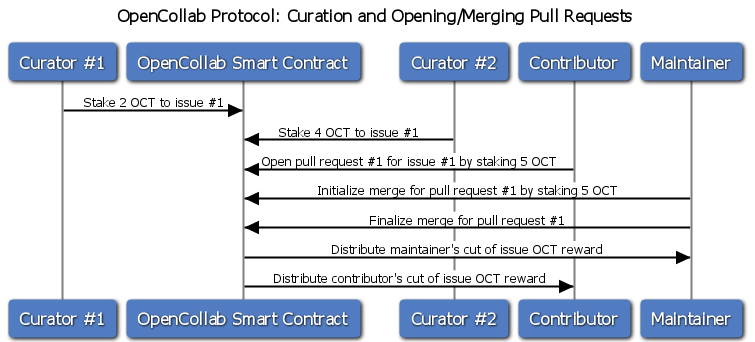
\includegraphics[width=\linewidth,keepaspectratio]{figures/OpenCollab-Protocol-Curation-And-Opening-Merging-Pull-Requests.png}
  \caption{Curating, opening pull requests and merging unchallenged pull requests}
\end{figure*}

\begin{figure*}[p!]
  \centering
  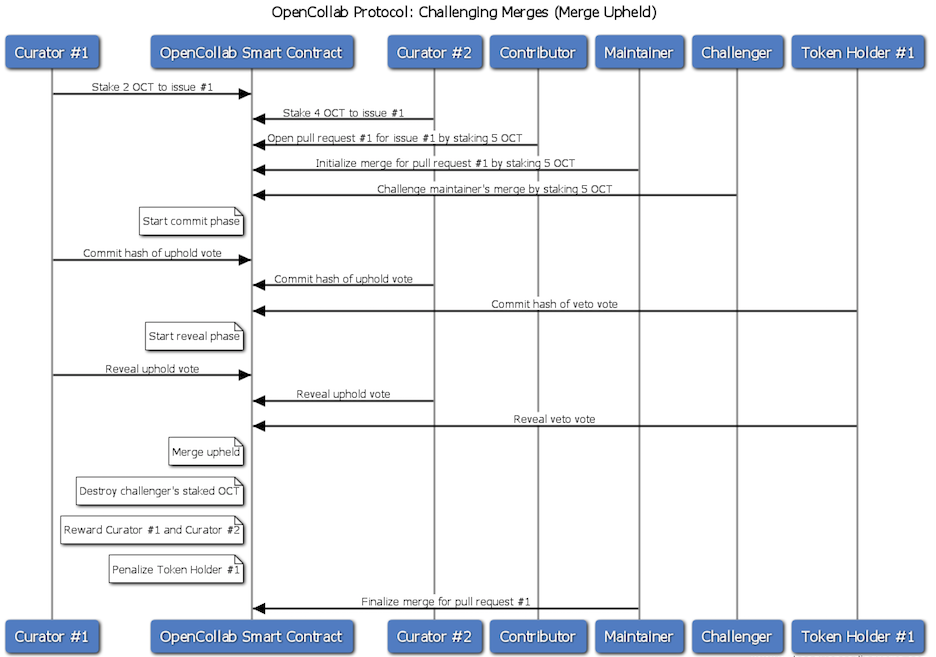
\includegraphics[width=\linewidth,keepaspectratio]{figures/OpenCollab-Protocol-Challenging-Merges-Upheld.png}
  \caption{Upholding a challenged merge}
\end{figure*}

\begin{figure*}[p!]
  \centering
  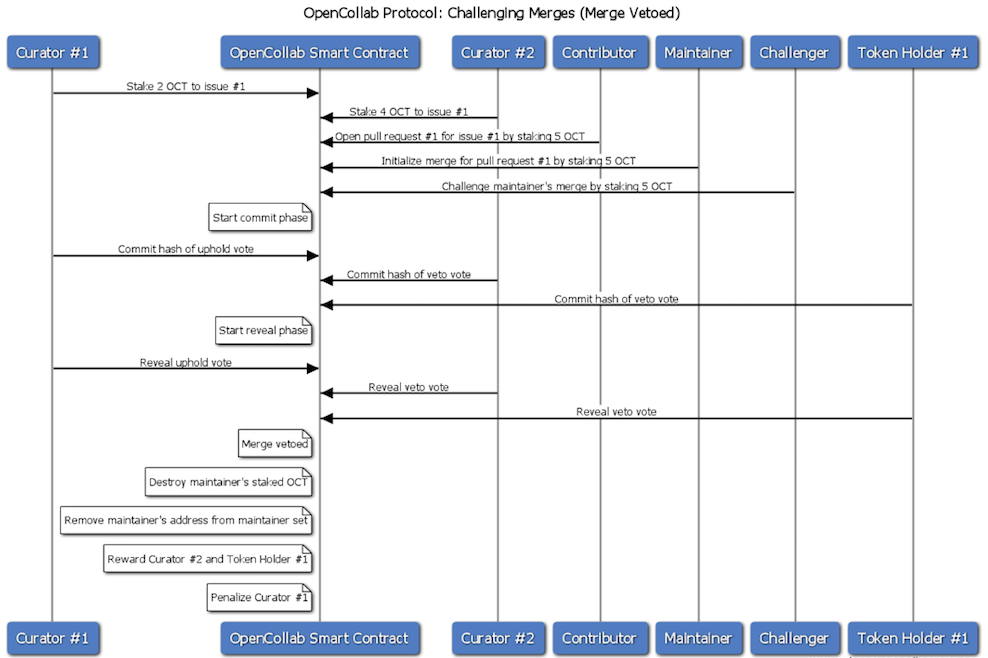
\includegraphics[width=\linewidth,keepaspectratio]{figures/OpenCollab-Protocol-Challenging-Merges-Veto.png}
  \caption{Vetoing a challenged merge}
\end{figure*}

\subsection{Amortisation of Work}

Each computation step taken by an Ethereum smart contract costs a certain amount
of gas, an internal accounting unit. As a result, when writing smart contracts,
it is important to keep in mind gas costs. One of the most costly programming
constructs that can be included in a smart contract is a loop over a large array
of elements. If the array of elements can become arbitrarily large, the gas cost
of iterating over the array can also become arbitrarily large.

In the OpenCollab protocol, voters are penalized or rewarded after a voting
round depending on whether they were on the winning or losing side of the vote.
A simple and naive way of performing the accounting for these penalties and
rewards would be to loop through all voters and check if they were on the
winning or losing side of the most recent vote. This accounting can be done at
the end of the \textproc{voteResult()} function.

However, the size of the voters array can become arbitrarily large as more token
holders put down despoits to participate in governance voting. As the voters
array grows in size, the gas cost of performing the accounting for penatlies and
rewards after a vote will grow as well. Accounting for penatlies and rewards in
such a way will eventually become too expensive.

A common design pattern used in smart contracts to avoid massive gas costs in
single function calls is amortisation of work\cite{amortisationWork}. We can
break up the work being done over other operations. In the OpenCollab protocol,
rather than updating voter deposits with penalties and rewards after every vote,
we introduce a \textproc{voterCheckIn()} function. The function updates a voter
deposit with penalties and rewards for all voting rounds that occured since the
last voting round that the voter checked in to.

Voters can only withdraw their deposits if they have checked in to the latest voting round. Voters are
incentivized to call \textproc{voterCheckIn()} frequently because otherwise the
gas cost of the function increases with the number of voting rounds that the
voter has not checked in. As a result, the work of calculating penalties and rewards for votes is distributed across
all voters and we avoid large gas costs associated with single function calls.

\subsection{Future Work}

\begin{figure*}
  \begin{minipage}{\textwidth}
    \begin{framed}
      \begin{lstlisting}
        // vr = latest voting round
        for (uint256 i = 0; i < voters.length; i++) {
          if(vr.votes[voters[i]].voteValue == VoteValue.None) {
            // Voter abstained
            // Penalize voter
          } else {
            if (vr.result == vr.votes[voters[i]].voteValue) {
              // Voter on winning side
              // Reward voter
            } else {
              // Voter on losing side
              // Penalize voter
            }
          }
        \end{lstlisting}
    \end{framed}
  \end{minipage}
  \caption{Calculating penalties and rewards for all voters in \textproc{voteResult()}}
\end{figure*}

\begin{figure*}
  \begin{minipage}{\textwidth}
    \begin{framed}
      \begin{lstlisting}
        for (uint i = startRound; i < rounds.length; i++) {
          if (rounds[i].votes[msg.sender].voteValue == VoteValue.None) {
            // Voter abstained
            // Penalize voter
          } else {
            if (rounds[i].result == rounds[i].votes[msg.sender].voteValue) {
              // Voter on winning side
              // Reward voter
            } else {
              // Voter on losing side
              // Penalize voter
            }
          }
        }
      \end{lstlisting}
    \end{framed}
  \end{minipage}
  \caption{Amorisation of work - voters calculate their own penalties and
    rewards in \textproc{voterCheckIn()}}
\end{figure*}

% Local Variables:
% org-ref-default-bibliography: ../bib/protocol.bib
% End:
